\section{Background}\label{sec:background}
\subsection{Gustavson's Method}\label{sec:gustav}
For a sparse matrix $X$, we define $n_X$, $m_X$, and $nnz_X$ as the number of rows, columns, and nonzero entries, respectively. The set $\mathcal{S}(X)$ denotes the column indices of all nonzero entries in $X$.
Our notation also extends to individual rows.
For example, for row $i$ of $X$, $nnz_{X_i}$ denotes the number of nonzero entries, and $\mathcal{S}(X_i)$ denotes the set of column indices corresponding to the nonzero entries.

The general sparse matrix-matrix multiplication operation (SpGEMM) is defined as $C=A B$, where $A$, $B$, and $C$ are sparse matrices.
Multithreaded implementations of SpGEMM are typically based on Gustavson's row-by-row algorithm~\cite{gustavson}:
\begin{equation}
    C_i = \sum_{j\in \mathcal{S}(A_i)} A_{ij}B_j,
    \label{equ:gustav}
\end{equation}
i.e., for some row $i$ of $C$, the rows of $B$ are scaled by the nonzero values in row $i$ of $A$.
These scaled rows are then summed together to give the final row of $C$.
Since each row of $C$ is computed independently, multithreaded implementations typically partition rows among threads,
which is the approach we take for MAGNUS.

There are two main ingredients for implementing Gustavson's method: the matrix storage scheme and the algorithm that \emph{accumulates} the scaled rows of $B$.
Compressed sparse row (CSR) format is one of the most popular storage schemes and is especially useful for algorithms such as Gustavson's method that traverse matrices row-wise. 
The CSR format requires three arrays: $C.col$, $C.val$, and $C.rowPtr$.
Arrays $C.col$ and $C.val$ of size $nnz_C$ store the column indices and values, respectively, of the nonzero entries of $C$, and $C.rowPtr$, of size $n_C+1$, stores the starting positions of each row in $C.col$ and $C.val$.

\autoref{alg:gustav_dense} shows the pseudocode for the \emph{numeric phase} of Gustavson's method. Variables in \textbf{bold} are global, meaning they are shared and visible across all threads.  
The scaled rows of $B$ are summed using a \emph{dense accumulator}, defined as the combination of \texttt{denseAccumBuff} and \texttt{bitMap}.
The column indices in row $i$ of $A$ are loaded as $idx = A.col[A.rowPtr[i]]$, and the rows of $B$ are loaded by reading $B.col$ from $B.rowPtr[idx]$ to $B.rowPtr[idx+1]$.
Array $denseAccumBuff$ of size $m_C$ is updated
for each column index of $B$, a companion bitmap stores the nonzero positions in $denseAccumBuff$, and $colBuff$ stores the running list of column indices in $C$.
Besides $A$, $B$, and $C$, all variables are thread-local.

\autoref{alg:gustav_dense} can be extended to other types of accumulators, e.g., hash map-based accumulators, where the dense accumulation array and bitmap are replaced by a hash map.
In other Gustavson-based algorithms, such as expand-sort-compress (ESC)~\cite{ESC,pbSpGEMM}, the \emph{intermediate product} of $C$ is written to an array instead of directly updating the accumulator.
This is shown in \autoref{alg:gustav_sort},
where the intermediate product is generated in the first loop by storing $B.col[k]$ and $A.val[j] \times  B.val[k]$ in 
$colBuff$ and $valBuff$, respectively.
The intermediate product is then sorted, duplicates are merged, and the result is written to $C$ (these steps take place in \texttt{sortMergeWrite(}$colBuff$,$valBuff$\texttt{)}).

\begin{algorithm}[htbp]
    \small
    \caption{Gustavson SpGEMM: Dense Accumulation}\label{alg:gustav_dense}
    \KwIn{$\bm{A}$, $\bm{B}$, $\bm{C.rowPtr}$}
    \KwOut{$\bm{C.col}$, $\bm{C.val}$}
    \SetCommentSty{emph}
    \DontPrintSemicolon
    \SetKwFor{ForPar}{for}{do \emph{in parallel}}{end forpar}
    \ForPar{$i \gets 0$\textbf{ to }$n-1$}{
        $count\gets 0$, $denseAccumBuff\gets 0$\;
        \text{\textbf{\color{blue}/* Read row $i$ of $A$ */}}\;
        \For{$j \gets \boldsymbol{A.rowPtr}[i]$\textbf{ to }$\boldsymbol{A.rowPtr}[i+1]-1$}{
            \text{\textbf{\color{blue}/* Read row $j$ of $B$ */}}\;
            \For{$k \gets \boldsymbol{B.rowPtr}[\boldsymbol{A.col}[j]]$\textbf{ to }$\boldsymbol{B.rowPtr}[\boldsymbol{A.col}[j]+1]-1$}{
                \text{\textbf{\color{blue}/* Multiply and update accumulator */}}\;
                $denseAccumBuff[\boldsymbol{B.col}[k]]$ \texttt{+=} $\boldsymbol{A.val}[j] \times  \boldsymbol{B.val}[k]$\;
                \If{$bitMap[\boldsymbol{B.col}[k]]$ \texttt{==} $0$}{
                    $colBuff[count\text{\texttt{++}}] \gets \boldsymbol{B.col}[k]$\;
                    $bitMap[\boldsymbol{B.col}[k]] \gets 1$\;
                }
            }
        }
        \text{\textbf{\color{blue}/* Write to $C$ */}}\;
        $k \gets \boldsymbol{C.rowPtr}[i]$\;
        \For{$j \in colBuff$}{
            $\boldsymbol{C.col}[k] \gets j$\;
            $\boldsymbol{C.val}[k\texttt{++}] \gets denseAccumBuff[j]$\;
            $bitMap[j] \gets 0$\;
        }
    }
\end{algorithm}

\begin{algorithm}[htbp]
    \small
    \caption{Gustavson SpGEMM: Expand-Sort-Compress (ESC)}\label{alg:gustav_sort}
    \KwIn{$\bm{A}$, $\bm{B}$, $\bm{C.rowPtr}$}
    \KwOut{$\bm{C.col}$, $\bm{C.val}$}
    \SetCommentSty{emph}
    \DontPrintSemicolon
    \SetKwFor{ForPar}{for}{do \emph{in parallel}}{end forpar}
    \ForPar{$i \gets 0$\textbf{ to }$n-1$}{
        $count\gets 0$\;
        \text{\textbf{\color{blue}/* Read row $i$ of $A$ */}}\;
        \For{$j \gets \boldsymbol{A.rowPtr}[i]$\textbf{ to }$\boldsymbol{A.rowPtr}[i+1]-1$}{
            \text{\textbf{\color{blue}/* Read row $j$ of $B$ */}}\;
            \For{$k \gets \boldsymbol{B.rowPtr}[\boldsymbol{A.col}[j]]$\textbf{ to }$\boldsymbol{B.rowPtr}[\boldsymbol{A.col}[j]+1]-1$}{
                \text{\textbf{\color{blue}/* Multiply and update accumulator */}}\;
               $colBuff[count] \gets \boldsymbol{B.col}[k]$\;
               $valBuff[count\text{\texttt{++}}] \gets \boldsymbol{A.val}[j] \times  \boldsymbol{B.val}[k]$\;
            }
        }
        \text{\textbf{\color{blue}/* Sort, merge, and write to $C$ */}}\;
        \texttt{sortMergeWrite(}$colBuff$,$valBuff$\texttt{)}\;
    }
\end{algorithm}

To compute $C.rowPtr$, which is an input to the numeric phase, an initial \emph{symbolic phase} is required.
The symbolic phase typically has the same high-level algorithm as the numeric phase but without performing the multiplication $A.val[j] \times  B.val[k]$ and writing to $C$.
For example, in \autoref{alg:gustav_dense}, the symbolic phase does not include the modifications to $denseAccumBuff$, $C.col$, and $C.val$.
Instead, only the bitmap is updated along with a counter that outputs the exact number of nonzero entries for each row of $C$.
Finally, $C.rowPtr$ is computed using a prefix sum on the counters.
This type of symbolic phase is known as \textit{precise prediction}, where the number of nonzero entries in $C$ is calculated exactly before the numeric phase.

\sloppy On modern CPUs, maximizing cache reuse is crucial to the performance of any application.
In SpGEMM, the accumulator is the most frequently accessed, where the amount of reuse is determined by the sparsity pattern of $A$ and $B$.
For optimal performance, the dense accumulator should be confined to the L2 cache, which is the highest level of private cache.
This efficient cache utilization occurs naturally in specific matrix structures, such as banded matrices or matrices that yield a highly sparse $C$. However, for matrices that produce ``large'' intermediate products (where ``large'' refers to both the number of nonzero elements and a wide distribution of column index values), SpGEMM faces significant challenges. A prominent example is random power-law matrices that model social networks~\cite{rmat}. For such matrices, the size of $denseAccumBuff$ often exceeds the capacity of the L2 cache and the large intermediate product results in frequent accesses to the entire $denseAccumBuff$ array. Consequently, $denseAccumBuff$ must frequently be evicted from and reloaded to the L2 cache, resulting in suboptimal performance. This breakdown in locality presents a substantial obstacle for current SpGEMM algorithms, as we will demonstrate through microbenchmarks and SpGEMM results.

\begin{figure*}[th]
\centering
\begin{tabular}{c}
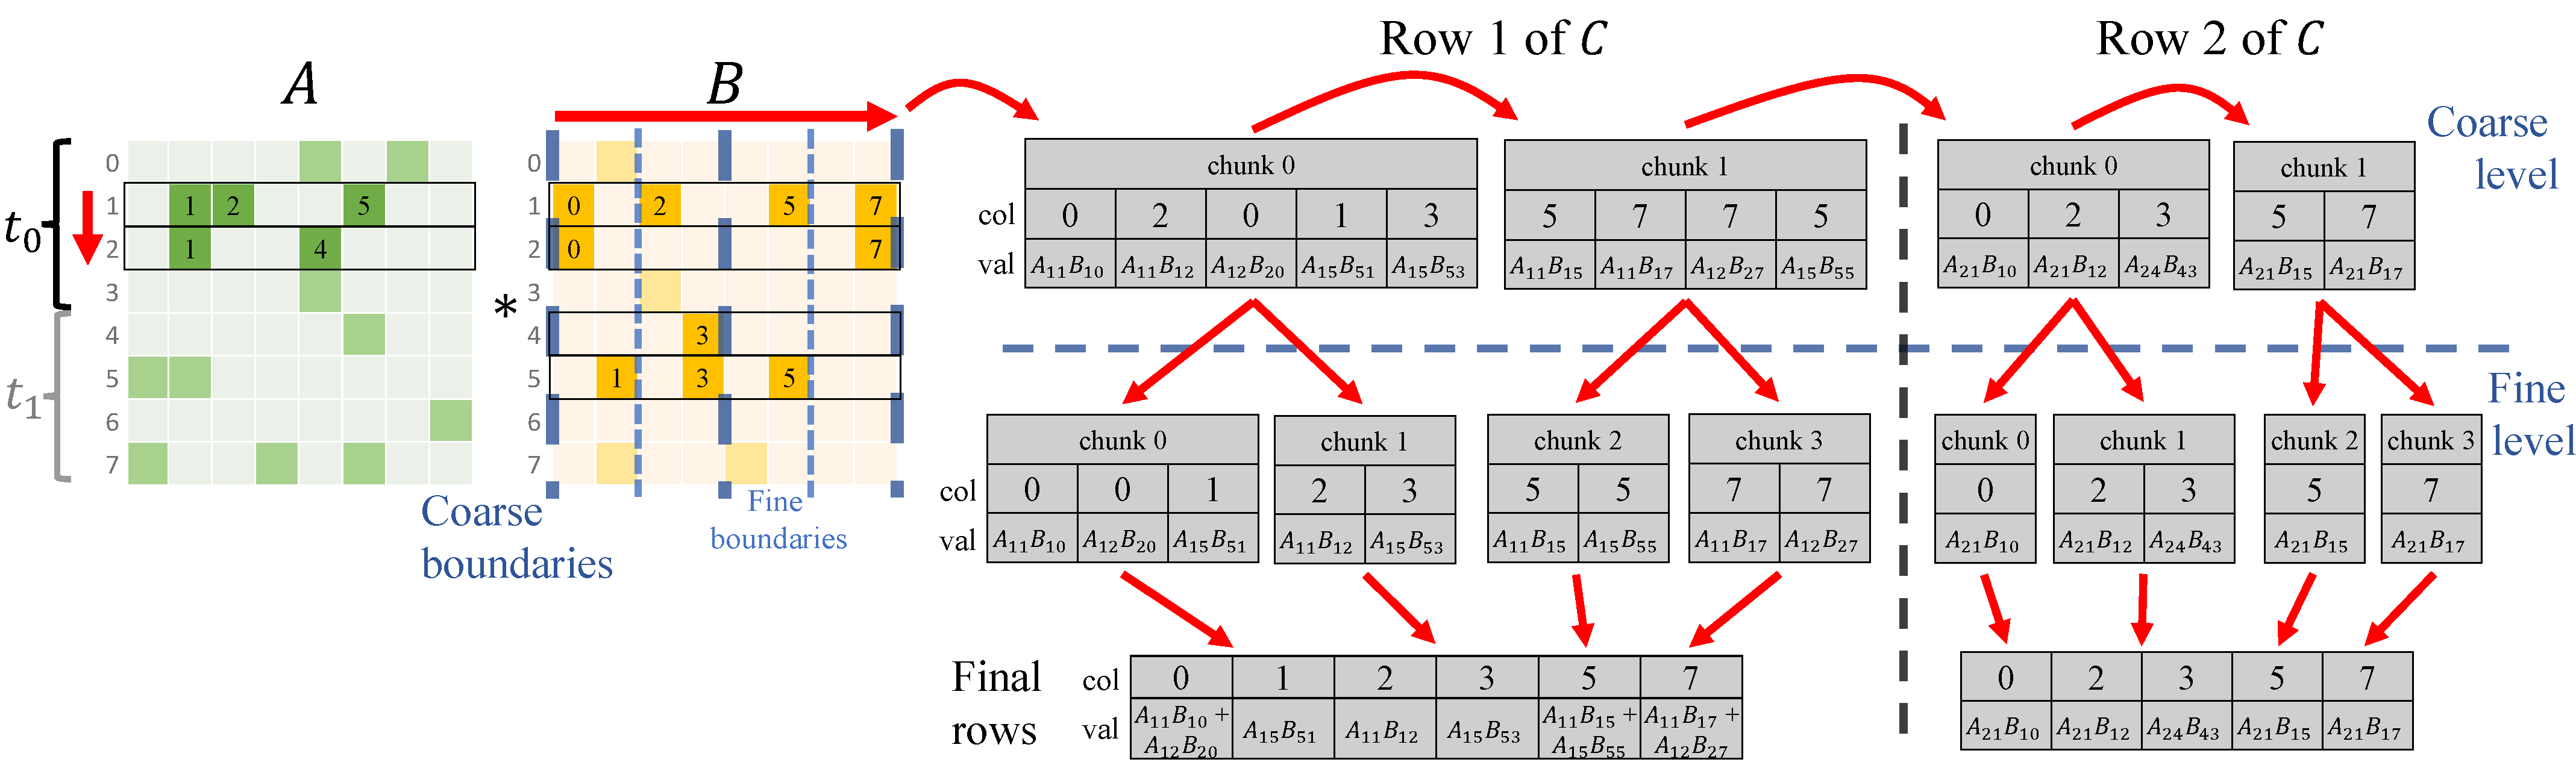
\includegraphics[width=\linewidth]{figs/MAGNUS_example_horizontal.pdf} 
\end{tabular}
\caption{Example workflow of MAGNUS, where two threads multiply two $8\times8$ matrices.
The computation of rows 1 and 2 assigned to thread $t_0$ is shown.
Two coarse- and fine-level chunks are used for each row.
}
\label{fig:MAGNUS_example}
\end{figure*}

\subsection{Related Work}
Optimizations related to the accumulation step have been the primary focus of research on SpGEMM.
For load balancing, a common approach is based on the observation that rows with different intermediate sizes require different accumulation strategies~\cite{liu1,liu2,ESC,pbSpGEMM,liu3,OpSparse,spECK,nagasaka3}.
In~\cite{ESC}, $A$ is reordered by increasing intermediate size.
Other approaches group rows based on the size of the intermediate product, where a different accumulator is used for different groups~\cite{liu1,liu2,liu3,OpSparse,spECK,nagasaka3,adaptLoadBalanceGPU}.
In~\cite{liu2}, five different accumulation strategies are used, including priority queues and sorting algorithms.
Developing new accumulators is another topic that has been widely studied, especially for modern multicore machines with vector processors~\cite{fevre,hierRowMerging,ASA,AVX512sort,nagasaka1,nagasaka2,gamma}.
A common approach is to optimize sorting algorithms~\cite{ESC,tricount3,liu1,AVX512sort,pbSpGEMM,registerAware}
or data structures such as heaps~\cite{azad,nagasaka1,nagasaka2} and hash maps~\cite{nagasaka1,nagasaka2,cuSPARSE,registerAware,mcl,balancedHashing,kokkos}.
In \autoref{sec:results_spgemm}, MAGNUS is compared with hash map and heap-based approaches, which are considered state-of-the-art~\cite{cseg,nagasaka1,nagasaka2,mkl}.


Perhaps most relevant to MAGNUS are recent works on improving the cache behavior of accumulators,
proposed in~\cite{partway} and improved in the CSeg method~\cite{cseg}.
The core concept is to partition the columns of $B$ into segments, where the number of segments is chosen so that the dense accumulator fits in the L2 cache.
An additional \emph{high-level summary matrix} is used to store the segmentation information. 
CSeg was shown to be overall faster than many state-of-the-art libraries mentioned above.
For a more extensive overview of SpGEMM research, including distributed memory algorithms, see~\cite{spgemmSurvey}.